\documentclass{article}

\usepackage[fleqn]{amsmath}
\usepackage{amssymb}
\usepackage{hyperref}
\usepackage{url}
\usepackage{graphicx}
\usepackage{geometry}
\usepackage{babel}
\usepackage{enumitem}
\usepackage{parskip}
\usepackage{chemfig}
\usepackage{pdfpages}
\usepackage{xcolor}
\usepackage{tikz}
\usepackage{fancybox}
\usepackage{makecell}
\usepackage{pgfplots}
\usepackage{soul}
\usepackage{ulem}
\usepackage{wrapfig}
\usepackage{subcaption}
\usepackage[T1]{fontenc}
\usepackage{esvect}
\usetikzlibrary{arrows}
\usetikzlibrary{decorations.pathreplacing}
\pgfplotsset{compat=1.17}
\definecolor{darkgreen}{rgb}{0.0, 0.6, 0.0}

\geometry{
    a4paper,
    total={170mm, 257mm},
    left=20mm,
    top=20mm
}

\hypersetup{
    colorlinks=true,
    linkcolor=black,
    urlcolor=blue,
    pdftitle={Mathematics 1A}
}

\newcommand{\figbox}[1]{ 
    \begin{figure*}[ht!]        
        \begin{center}            
            \fbox{#1}        
        \end{center}    
    \end{figure*}
}

\newcommand{\wrapfill}{
    \par
    \ifnum \value{WF@wrappedlines} > 0
        \addtocounter{WF@wrappedlines}{-1}%
        \null\vspace{
            \arabic{WF@wrappedlines}
            \baselineskip
        }
        \WFclear
    \fi
    \phantom{}
}

\newcommand{\difference}{\,\backslash\,}
\newcommand{\rem}{\underline{Remark}: }
\newcommand{\nots}{\underline{Notation}: }
\newcommand{\prf}{\underline{Proof}: }
\newcommand{\exs}{\underline{Example}: }
\newcommand{\defs}{\underline{Definition}: }
\newcommand{\wrn}{\underline{Warning}: }
\newcommand{\sht}{\ |\ }
\newcommand{\pph}[1]{\paragraph{#1} \phantom{}\\}
\newcommand{\dm}{\displaystyle}

% === TEXT ===
\title{\textbf{Mathematics 1A \\ HSLU, Semester 1}}
\author{Matteo Frongillo}

\begin{document}

\maketitle
\tableofcontents
\pagebreak

\part{Week 1}
\section{The set theory}
\subsection{Definition of a set}
A set is a collection of objects or elements.

\rem{The collection of all sets is not a set.}

\subsection{Logical symbols}
\subsubsection{Definition}
Braces and the definition symbol ``$:=$'' are used to define a set giving all its elements:
\figbox{$A:=\left\{a,b,c,d,e\right\}$}

\subsubsection{Equal}
In this case, the equal symbol means that the set $A$ is equal to the set $B$:
\figbox{$A=B$}

\subsubsection{Belongs to}
The symbols $\in$ and $\ni$ describe an element which is part of the set:
\figbox{$a \in A \Longleftrightarrow A \ni a$}

\subsubsection{Does not belong to}
The symbols $\notin$ mean that an element does not belong to the set:
\figbox{$f \notin A$}

\subsubsection{Inclusion and contains}
The symbols $\subset$ and $\supset$ mean that a set has another set included in its set:
\figbox{$\mathbb{N} \subset \mathbb{Z} \Longleftrightarrow \mathbb{Z} \supset \mathbb{N}$}

\subsubsection{For all/any}
The symbol $\forall$ means that we are considering any type of element:
\figbox{$\forall x \in \mathbb{R},\ x>0$}

In this case, we've defined a new set.

\subsection{Numerical sets}
\begin{itemize}
    \item $\mathbb{N} :=$ Natural numbers (including 0);
    \item $\mathbb{Z} :=$ Integer numbers;
    \item $\mathbb{Q} :=$ Rational numbers;
    \item $\mathbb{R} := \text{Real numbers} := \mathbb{Q} \cup \left\{\text{irrational numbers}\right\}.$
\end{itemize}

\nots{The ``$^*$'' symbol means that the set does not include 0.}

\subsubsection{Inclusion of sets}
\figbox{$\mathbb{N} \subset  \mathbb{Z} \subset \mathbb{Q} \subset \mathbb{R} \subset \mathbb{C}$}

$
    B := \left\{\pi, 1,-1,0\right\}; \\
    C := \left\{\pi, 1\right\}; \\
    D := \left\{\pi\right\}.
$

Then we write some examples: $\pi \in B,\ D \subset B,\ C \subset B,\ B \not\subset C,\ 0 \in B,\ 0 \notin C$.

\section{Intervals in the real line}
Intervals describe what happens between two or more elements.

\subsection{Examples}
\subsubsection{Interval sets}
We have 4 cases:
\begin{itemize}
    \item $(a,b) = \left\{\forall x \in \mathbb{R} \sht a<x<b\right\}$;
    \item $\left[a,b\right) = \left\{\forall x \in \mathbb{R} \sht a\leq x<b\right\}$;
    \item $\left(a,b\right] = \left\{\forall x \in \mathbb{R} \sht a<x\leq b\right\}$;
    \item $\left[a,b\right] = \left\{\forall x \in \mathbb{R} \sht a\leq x\leq b\right\}$.
\end{itemize}

\nots{$a$ and $b$ are often called the ``end points'' of the interval;\\}

\subsubsection{Graphical examples}
$\forall x \in \mathbb{R},\ x \in \left[a,b\right]$
\begin{center}
    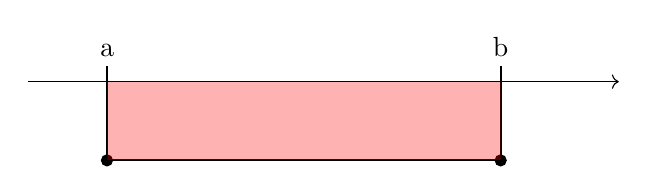
\begin{tikzpicture}
        %number line
        \draw[-] (-4,0) -- (3,0);
        \draw[thick] (-3,-0.2) -- (-3,0.2);
        \draw[thick] (2,-0.2) -- (2,0.2);
        
        %interval
        \draw[thick] (-3,-1) -- (2,-1);
        \draw[thick] (-3,0) -- (-3,-1);
        \draw[thick] (2,0) -- (2,-1);
        \filldraw[black] (-3,-1) circle (2pt);
        \filldraw[black] (2,-1) circle (2pt);
        
        %points
        \node[above] at (-3,0.2) {a};
        \node[above] at (2,0.2) {b};
        
        %arrow
        \draw[->] (3,0) -- (3.5,0);

        %area
        \filldraw [fill=red, draw=black, opacity=0.3] (-3,0) rectangle (2,-1);
    \end{tikzpicture}
\end{center}

\newpage
\section{The extended line}
In the real line $\mathbb{R}$ we add $\pm \infty$.

\paragraph{Real line:} $(-\infty, +\infty) = \mathbb{R}$ 

\paragraph{Extended real line:} $\left[-\infty, +\infty\right] = \overline{\mathbb{R}}$

\vspace*{.5cm}
\begin{center}
    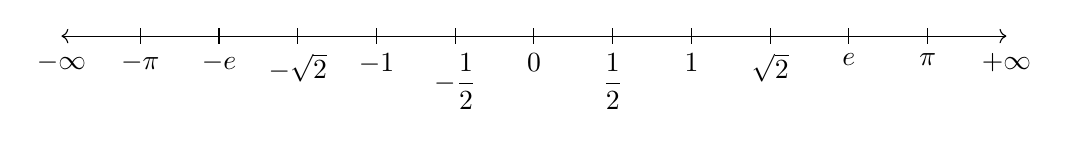
\begin{tikzpicture}
        \draw[->] (0,0) -- (6,0);
        \draw[<-] (-6,0) -- (0,0);

        \foreach \x/\label in {-5/{$-\pi$}, -4/{$-e$}, -3/{$-\sqrt{2}$}, -2/{$-1$}, -1/{$-\dfrac{1}{2}$}, 0/{$0$}, 1/{$\dfrac{1}{2}$}, 2/{$1$}, 3/{$\sqrt{2}$}, 4/{$e$}, 5/{$\pi$}} {
            \draw (\x,0.1) -- (\x,-0.1) node[below] {\label};
        }
        \node[below] at (-6,-0.1) {$-\infty$};
        \node[below] at (6,-0.1) {$+\infty$};
    \end{tikzpicture}
\end{center}

\rem{$\pm \infty \notin \mathbb{R}$}

\subsection{Properties}
\figbox{$\forall x \in \mathbb{R} \ \sht \ \infty > x \ \sht \ -\infty < 0$}

\subsection{Operation in the extended line}
If $a,b \in \mathbb{R}$, then $a+b,\; a-b,\; a\cdot b,\; \dfrac{a}{b} \text{ (with } b\neq 0 )$ stay the same

\subsubsection{Additions}
Let $\forall a \in \mathbb{R}$:
\begin{itemize}
    \item $a+\infty := \infty$;
    \item $a-\infty := -\infty$;
    \item $+\infty + \infty := +\infty$;
    \item $-\infty - \infty := -\infty$;
    \item $+\infty - \infty :=$ undefined.
\end{itemize}

\subsubsection{Moltiplications}
Let $\forall a \in \mathbb{R}$:
\begin{itemize}
    \item $+\infty \cdot +\infty := +\infty$;
    \item $-\infty \cdot +\infty := -\infty$;
    \item $-\infty \cdot (-\infty) := \infty$;
    \item $a \cdot \infty := \begin{cases}
        a > 0 &+\infty\\
        a < 0 &-\infty\\
        a = 0 & \text{undefined}
    \end{cases}$
    \item $a \cdot (-\infty):= \begin{cases}
        a > 0 &-\infty\\
        a < 0 &+\infty\\
        a = 0 &\text{undefined}
    \end{cases}$
    \item $\dfrac{a}{+\infty}=\dfrac{a}{-\infty} := 0$;
    \item $\dfrac{+\infty}{a}:= \begin{cases}
        a > 0 &+\infty\\
        a < 0 &-\infty\\
        a = 0 &+\infty
    \end{cases}$
    \item $\dfrac{-\infty}{a}:= \begin{cases}
        a > 0 &-\infty\\
        a < 0 &+\infty\\
        a = 0 &-\infty
    \end{cases}$
    \item $\dfrac{\infty}{\infty}:=$ undefined.
\end{itemize}

\section{Intervals including $\pm \infty$}
Intervals describe what happens between two or more elements, including $\pm \infty$.
\subsection{Examples}
\subsubsection{Interval sets}
Let $a \in \mathbb{R}$, then:
\begin{itemize}
    \item $(-\infty,a)=\left\{\forall x \in \mathbb{R} \sht x < a\right\}$;
    \item $(a, +\infty)=\left\{\forall x \in \mathbb{R} \sht x > a\right\}$;
    \item $(-\infty, a]=\left\{\forall x \in \mathbb{R} \sht x \leq a\right\}$;
    \item $[a,+\infty]=\left\{\forall x \in \mathbb{R} \sht x \geq a\right\}$;
    \item $(-\infty,+\infty)=\mathbb{R}$;
    \item $[-\infty,+\infty]=\overline{\mathbb{R}}$.
\end{itemize}

\subsubsection{Graphical examples}
$\forall x \in \mathbb{R},\ x \in\ \left[a,b\right]\ \cup\ \left] c, +\infty\right[$

\begin{center}
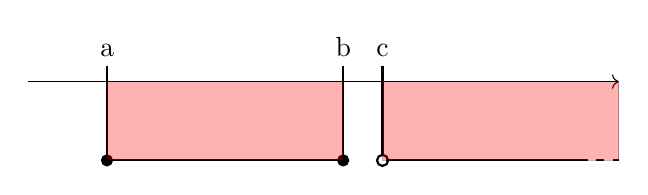
\begin{tikzpicture}
    %number line
    \draw[-] (-3,0) -- (4,0);
    \draw[thick] (-2,-1) -- (-2,0.2);
    \draw[thick] (1,-1) -- (1,0.2);
    \draw[thick] (1.5,-0.95) -- (1.5,0.2);
    
    %intervals
    \draw[thick] (-2,-1) -- (1,-1);
    \filldraw[black] (-2,-1) circle (2pt);
    \filldraw[black] (1,-1) circle (2pt);
    \draw[thick] (1.55,-1) -- (4,-1);
    \draw[thick, dashed] (4,-1) -- (4.5,-1);
    \draw[thick] (1.5,-1) circle (2pt);
    
    %points
    \node[above] at (-2,0.2) {a};
    \node[above] at (1,0.2) {b};
    \node[above] at (1.5,0.2) {c};
    
    %arrow
    \draw[->] (4,0) -- (4.5,0);

    %area
    \filldraw [fill=red, draw=black, opacity=0.3] (-2,0) rectangle (1,-1);
    \filldraw [fill=red, draw=black, opacity=0.3] (1.5,0) rectangle (4.5,-1);
\end{tikzpicture}
\end{center}
\vspace*{.5cm}
\nots{The union of two or more intervals where $x \in \mathbb{R}$
is denoted by the symbol $\cup$.}

\section{Propositional logic}
Propositional logic is a branch of mathematics that deals with propositions and logical operations.

\subsection{Logical connectives}
\begin{center}
    \begin{tabular}{|c|c|c|c|c|c|c|}
        \hline \rule{0pt}{15pt}
        A & B & $\lnot B$ & $A \land B$ & $A \lor B$ & $A \Rightarrow B$ & $A \Leftrightarrow B$ \\
        \hline \rule{0pt}{15pt} T & T & F & T & T & T & T \\
        \hline \rule{0pt}{15pt} T & F & T & F & T & F & F \\
        \hline \rule{0pt}{15pt} F & T & F & F & T & T & F \\
        \hline \rule{0pt}{15pt} F & F & T & F & F & T & T \\
        \hline
    \end{tabular}
\end{center}

\subsubsection{Logical conjunction $\land$}
Given two statements $P$ and $Q$, $P \land Q$ is true if both $P$ and $Q$ are true.

Let $P=(x>0)$ and $Q=(y>0)$, then:
\figbox{$P \land Q = (x > 0 \land y > 0)$}

\subsubsection{Logical disjunction $\lor$}
Given two statements $P$ and $Q$, $P \lor Q$ is true if at least one of $P$ or $Q$ is true.

Let $P=(x=0)$ and $Q=(y \neq 0)$, then:
\figbox{$P \lor Q = (x = 0 \lor y \neq 0)$}

\subsubsection{Logical negation $\lnot$}
The negation of a statement $P$, denoted as $\lnot P$, is true if $P$ is false, and false if $P$ is true.

Let $P=(x \geq 5)$, then:
\figbox{$\lnot P = (x < 5)$}

\subsubsection{Implication $\Rightarrow$}
The symbol $\Rightarrow$ indicates that if statement $P$ is true, then statement $Q$ must also be true (i.e., $P$ implies $Q$).\\
\wrn{It does not require that $Q$ implies $P$.}

\figbox{$P=(x=1) \Rightarrow Q = (x \in \mathbb{N})$}

\subsubsection{Inference $\Leftarrow$}
The symbol $\Leftarrow$ means that a conclusion or result implies the truth of an earlier statement.\\
If $Q$ is true, then $P$ must be true.

\figbox{$Q = (x > 0) \Leftarrow P = (x \in \mathbb{R}^+)$}

\subsubsection{If and only if $\Leftrightarrow$}
The symbol $\Leftrightarrow$ indicates that two statements $P$ and $Q$ are logically equivalent, meaning $P$ is true if and only if $Q$ is true.
\figbox{$P = (x \in \mathbb{N},\ x \neq 0) \Longleftrightarrow Q = (x \in \mathbb{N}^*)$}

\section{Union $\cup$ and Intersection $\cap$}
\subsection{Universe symbol}
The symbol $\bigcup :=$ Universe describes a big set which contains all sets involved
in our discussions (not always).

\subsection{Venn diagram}
\subsubsection{Union $A \cup B$}
If $A$ and $B$ are sets, then their union is:
\figbox{$A \cup U = \left\{\forall x \in \bigcup \sht x \in A \lor x \in B\right\}$}
\vspace*{-.53cm}
\figbox{
    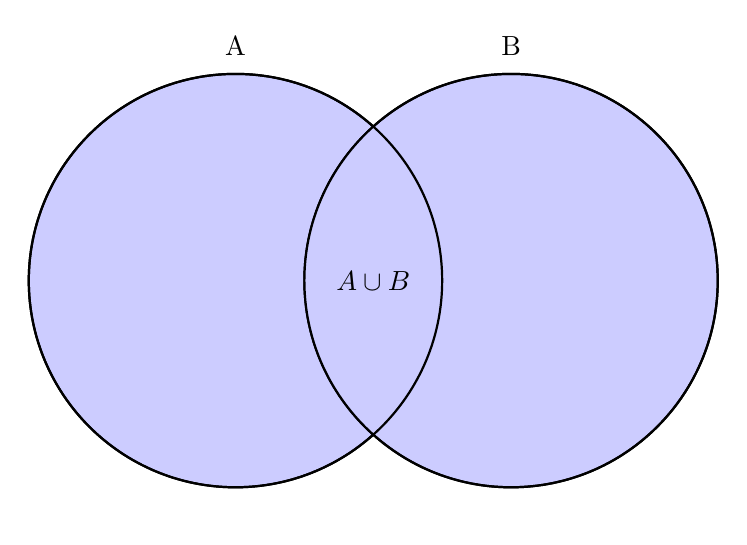
\begin{tikzpicture}[scale=1.75]
        \draw[thick, fill=blue!20] (2, 2) circle (1.5);
        \draw[thick, fill=blue!20] (4, 2) circle (1.5);
        
        \begin{scope}
            \clip (2, 2) circle (1.5);
            \fill[white] (4, 2) circle (1.5);
            \clip (2, 2) circle (1.5);
            \fill[blue!20] (4, 2) circle (1.5);
        \end{scope}

        \draw[thick] (2, 2) circle (1.5);
        \draw[thick] (4, 2) circle (1.5);
        
        \node at (2, 3.7) {A};
        \node at (4, 3.7) {B};
        
        \node at (3, 2) {\(A \cup B\)};
        
        \node at (3, 0.35) {};

        \node[overlay] at (0.2,3.75) {\(\bigcup\)};
    \end{tikzpicture}
}

\newpage
\subsubsection{Intersection $A \cap B$}
If $A$ and $B$ are sets, then their intersection is:
\figbox{$A \cap B = \left\{\forall x \in \bigcup \sht x \in A \land x \in B\right\}$}

\figbox{
    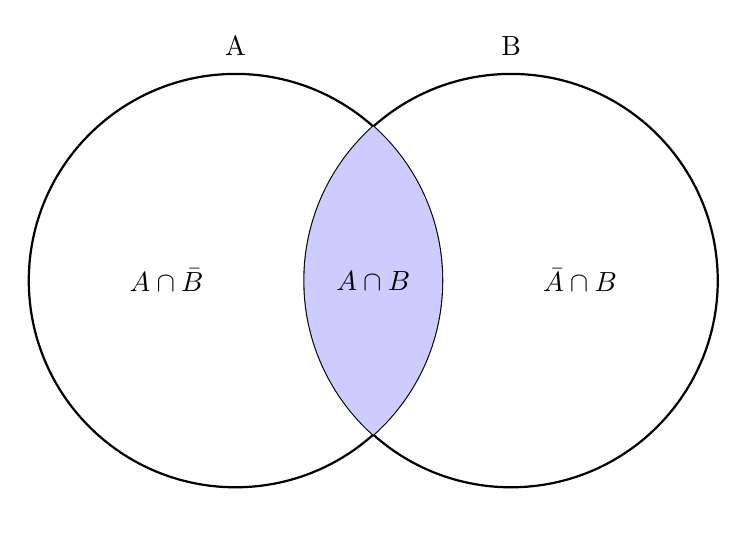
\begin{tikzpicture}[scale=1.75]
        
        \draw[thick] (2, 2) circle (1.5);
        \draw[thick] (4, 2) circle (1.5);
        \begin{scope}
            \clip (2, 2) circle (1.5);
            \fill[blue!20] (4, 2) circle (1.5);
        \end{scope}
        
        \node at (2, 3.7) {A};
        \node at (4, 3.7) {B};
        
        \node at (1.5, 2) {\(A \cap \bar{B}\)};
        \node at (4.5, 2) {\(\bar{A} \cap B\)};
        \node at (3, 2) {\(A \cap B\)};
        
        \node at (3, 0.35) {};

        \node[overlay] at (0.2,3.75) {\(\bigcup\)};
    \end{tikzpicture}
}

\subsubsection{Complement $\bar{A}$}
If $A$ is a set, its complement is:
\figbox{$\bar{A}=\left\{\forall x \in \bigcup \sht x \notin A\right\}$}

\begin{figure}[ht!]
    \begin{center}
            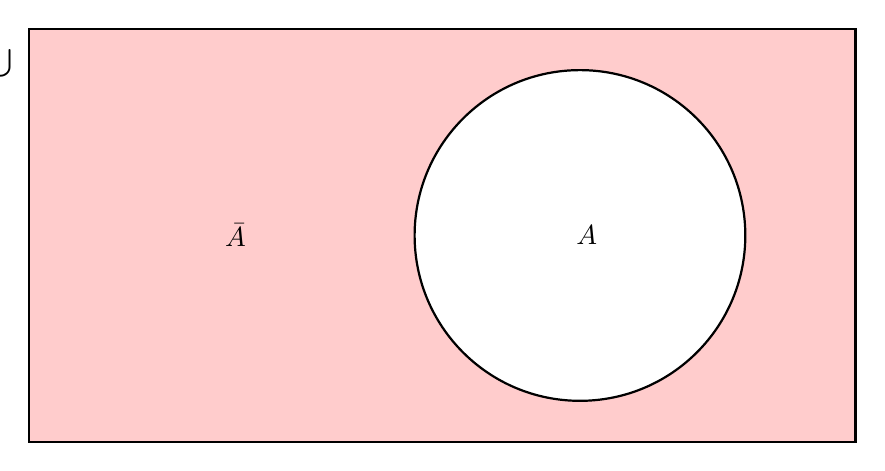
\begin{tikzpicture}[scale=1.75]
                
                \fill[red!20] (0, 0) rectangle (6, 3);
                \draw[thick] (0, 0) rectangle (6, 3);
        
                \fill[white] (4, 1.5) circle (1.2);
                \draw[thick] (4, 1.5) circle (1.2);
                
                \node at (1.5, 1.5) {\(\bar{A}\)};
                \node at (4.05, 1.5) {\(A\)};

                \node[overlay] at (-0.2,2.75) {\(\bigcup\)};
            \end{tikzpicture}
    \end{center}
\end{figure}

\newpage
\subsubsection{Difference between sets $\difference$}
If $A$ and $B$ are sets, then their difference is:
\figbox{$A \difference B = \left\{\forall x \in \bigcup \sht x \in A,\ x \notin B\right\}$}

\figbox{        
    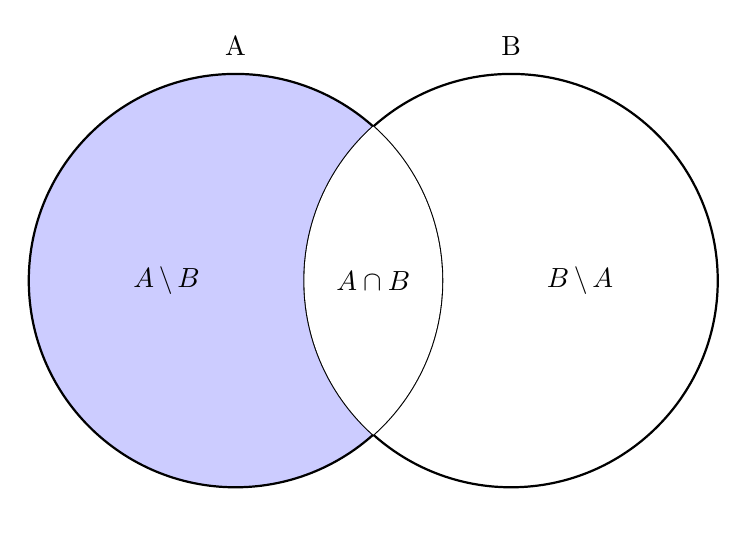
\begin{tikzpicture}[scale=1.75]
        \draw[thick, fill=blue!20] (2, 2) circle (1.5);
        \draw[thick] (4, 2) circle (1.5);
            
        \begin{scope}
            \clip (2, 2) circle (1.5);
            \fill[white] (4, 2) circle (1.5);
        \end{scope}
        
        \node at (2, 3.7) {A};
        \node at (4, 3.7) {B};
        
        \node at (1.5, 2) {\(A \difference B\)};
        \node at (4.5, 2) {\(B \difference A\)};
        \node at (3, 2) {\(A \cap B\)};
        
        \node at (3, 0.35) {};

        \node[overlay] at (0.2,3.75) {\(\bigcup\)};
    \end{tikzpicture}
}

\subsubsection{Symmetrical difference $\bigtriangleup$}
If $A$ and $B$ are sets, then their symmetrical difference is:
\figbox{$A \bigtriangleup B = (A \setminus B) \cup (B \setminus A)$}
\figbox{
    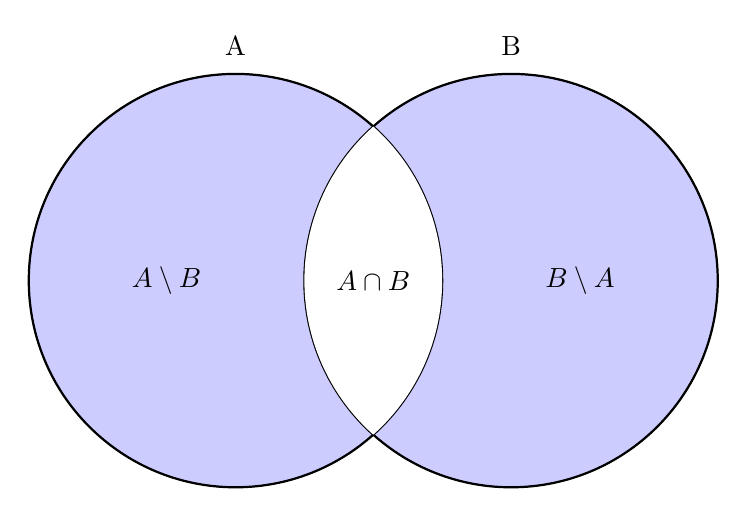
\begin{tikzpicture}[scale=1.75]
        \draw[fill=blue!20] (2, 2) circle (1.5);
        \draw[fill=blue!20] (4, 2) circle (1.5);
        
        \draw[thick] (2, 2) circle (1.5);
        \draw[thick] (4, 2) circle (1.5);
        
        \begin{scope}
            \clip (2, 2) circle (1.5);
            \fill[white] (4, 2) circle (1.5);
        \end{scope}
        
        \node at (2, 3.7) {A};
        \node at (4, 3.7) {B};
        
        \node at (1.5, 2) {\(A \setminus B\)};
        \node at (4.5, 2) {\(B \setminus A\)};
        \node at (3, 2) {\(A \cap B\)};
    \end{tikzpicture}
}

\newpage
\subsubsection{Disjoined sets (Empty sets) $\emptyset$}
$\emptyset :=$ the set containing zero elements:
\figbox{$A \cap B = \emptyset$}

\begin{figure}[ht!]
    \begin{center}
            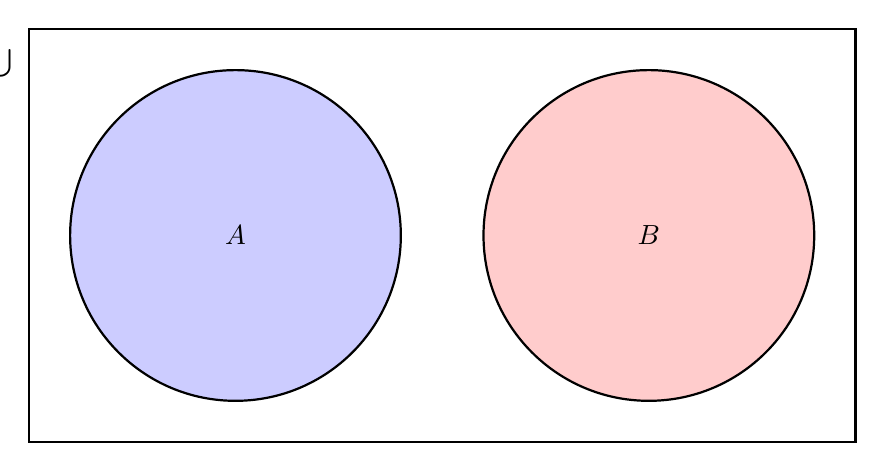
\begin{tikzpicture}[scale=1.75]
                
                \draw[thick] (0, 0) rectangle (6, 3);
        
                \fill[blue!20] (1.5, 1.5) circle (1.2);
                \draw[thick] (1.5, 1.5) circle (1.2);
                \fill[red!20] (4.5, 1.5) circle (1.2);
                \draw[thick] (4.5, 1.5) circle (1.2);
                
                \node at (1.5, 1.5) {\(A\)};
                \node at (4.5, 1.5) {\(B\)};
                            
                \node[overlay] at (-0.2,2.75) {\(\bigcup\)};
            \end{tikzpicture}
    \end{center}
\end{figure}

\section{The absolute value function}
The absolute value is an operator that returns the positive value of a
number, regardless of its original sign.

Let $x \in \mathbb{R}$, then:
\figbox{$|x|=\begin{cases}
    x \text{ if} &x \geq 0\\
    x \text{ if} &-x < 0
\end{cases}$}

\subsection{Graph of absolute value functions}
Let's plot the function $y=|x|$:
\begin{figure}[ht!]
    \centering
    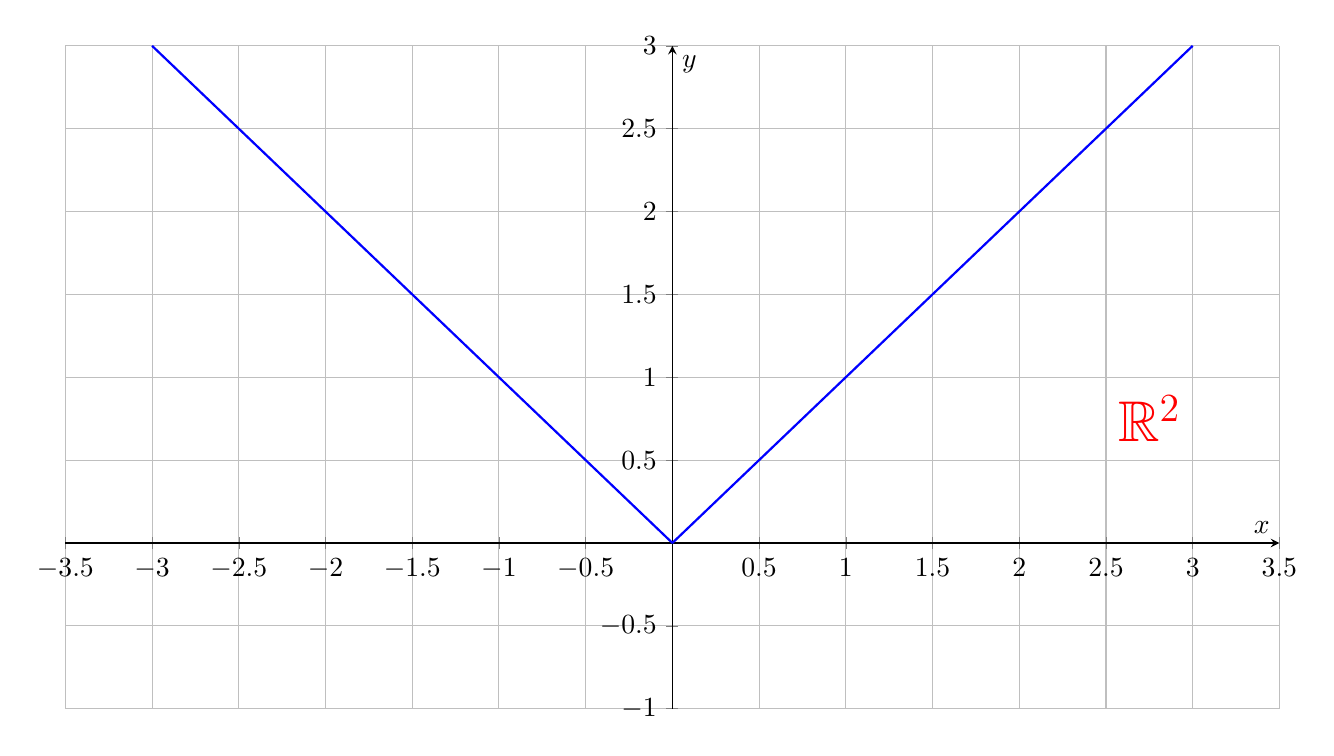
\begin{tikzpicture}
        \begin{axis}[
            axis lines = middle,
            xlabel = {$x$},
            ylabel = {$y$},
            domain=-3:3,
            samples=1500,
            xmin=-3.5, xmax=3.5,
            ymin=-1, ymax=3,
            grid=major,
            width=17cm, height=10cm
        ]
            \addplot[blue, thick] {abs(x)};
            \node[red] at (2.75,.75) {\huge $\mathbb{R}^2$};
            \end{axis}
    \end{tikzpicture}
\end{figure}

\subsection{Properties}
Let $a,b \in \mathbb{R}$, then:
\begin{itemize}
    \item $|a\cdot b|=|a| \cdot |b|$;
    \item $\left\vert\dfrac{a}{b}\right\vert= \dfrac{|a|}{|b|} $ for $b \neq 0$;
    \item $|a\pm b| \neq |a|\pm |b|$.
\end{itemize}

\subsection{Triangular inequalities}
Let $a,b \in \mathbb{R}$, then:
\figbox{\begin{minipage}{0.135\textwidth}
    \begin{center}
        $|a|+|b| \geq |a+b|$\\
        $|a|-|b| \leq |a-b|$ 
    \end{center}
\end{minipage}
}

\newpage
\part{Week 2}
\section{Concept of functions}
Let's take any two sets $A\left\{a,b,c,d,e,f,g\right\}$ and $B\left\{a_1,b_1,c_1,d_1,e_1,f_1,g_1\right\}$.

\figbox{ \hspace*{-1cm}
    \begin{minipage}{0.12\textwidth}
        \vspace*{-0.4cm}
        \begin{align*}
            f: A &\rightarrow B \\
            a &\longmapsto f(a)
        \end{align*}
    \end{minipage}
}

A function is a relation between the sets $A$ and $B$, according to which we
associate to each element of $A$ one and only one element of $B$:

\figbox{
    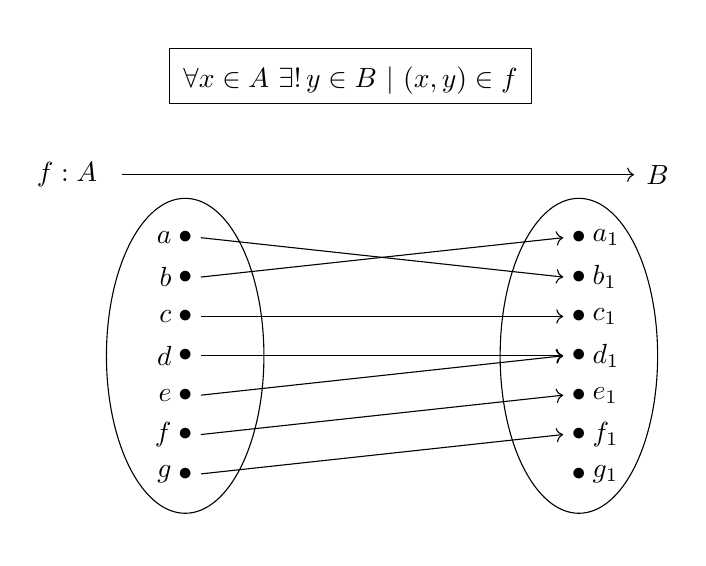
\begin{tikzpicture}

        %formula
        \node at (2.1,3.5) {$\forall x \in A\ \exists!\, y \in B \sht (x,y) \in f$};
        \draw (-0.2,3.2) rectangle (4.4,3.9);

        %sets A and B
        \draw (0,0) ellipse (1 and 2);
        \draw (5,0) ellipse (1 and 2);
        \node at (-1.5,2.3) {$f:A$};
        \node at (6,2.3) {$B$};
        \draw[->] (-0.8,2.3) -- (5.7,2.3);
        
        %set A
        \node at (0,-1.5) {$\bullet$};
        \node[left] at (-0.05,-1.5) {$g$};
        \node at (0,-1) {$\bullet$};
        \node[left] at (-0.05,-1) {$f$};
        \node at (0,-0.5) {$\bullet$};
        \node[left] at (-0.05,-0.5) {$e$};
        \node at (0,0) {$\bullet$};
        \node[left] at (-0.05,0) {$d$};
        \node at (0,0.5) {$\bullet$};
        \node[left] at (-0.05,0.5) {$c$};
        \node at (0,1) {$\bullet$};
        \node[left] at (-0.05,1) {$b$};
        \node at (0,1.5) {$\bullet$};
        \node[left] at (-0.05,1.5) {$a$};
        
        %set B
        \node at (5,-1.5) {$\bullet$};
        \node[right] at (5.05,-1.5) {$g_1$};
        \node at (5,-1) {$\bullet$};
        \node[right] at (5.05,-1) {$f_1$};
        \node at (5,-0.5) {$\bullet$};
        \node[right] at (5.05,-0.5) {$e_1$};
        \node at (5,0) {$\bullet$};
        \node[right] at (5.05,0) {$d_1$};
        \node at (5,0.5) {$\bullet$};
        \node[right] at (5.05,0.5) {$c_1$};
        \node at (5,1) {$\bullet$};
        \node[right] at (5.05,1) {$b_1$};
        \node at (5,1.5) {$\bullet$};
        \node[right] at (5.05,1.5) {$a_1$};
        
        %arrows
        \draw[->] (0.2,-1.5) -- (4.8,-1);
        \draw[->] (0.2,-1) -- (4.8,-0.5);
        \draw[->] (0.2,-0.5) -- (4.8,0);
        \draw[->] (0.2,0) -- (4.8,0);
        \draw[->] (0.2,0.5) -- (4.8,0.5);
        \draw[->] (0.2,1) -- (4.8,1.5);
        \draw[->] (0.2,1.5) -- (4.8,1);

        %spacer
        \node at (0,4.05) {\phantom{}};
        \node at (0,2.6) {\phantom{}};
        \node at (0,-2.2) {\phantom{}};
    \end{tikzpicture}
}

\nots{$f(a)=b_1,\ f(b)=a_1,\ f(c)=c_1,\ f(d)=d_1,$ ...}

Each point in set $A$ is associated with one element of $B$. However, it is
possible for more than two elements of $A$ to point to the same element of $B$.

\figbox{The set $A$ is called \textit{domain} of $f$. The set $B$ is called the \textit{codomain} of $f$.}

\subsection{Image (Range)}
Let $f: X \rightarrow Y$ be a function. The image of $f$ is defined as:
\figbox{\text{Im($f$)}$=\{y \in Y \sht y=f(x),\ x \in X\}$}

Easily, the image is the set containing all the elements of the set $B$ associated
with the elements of the set $A$.

\newpage
\section{Linear function}
\subsection{Cartesian diagram}
\begin{center}
    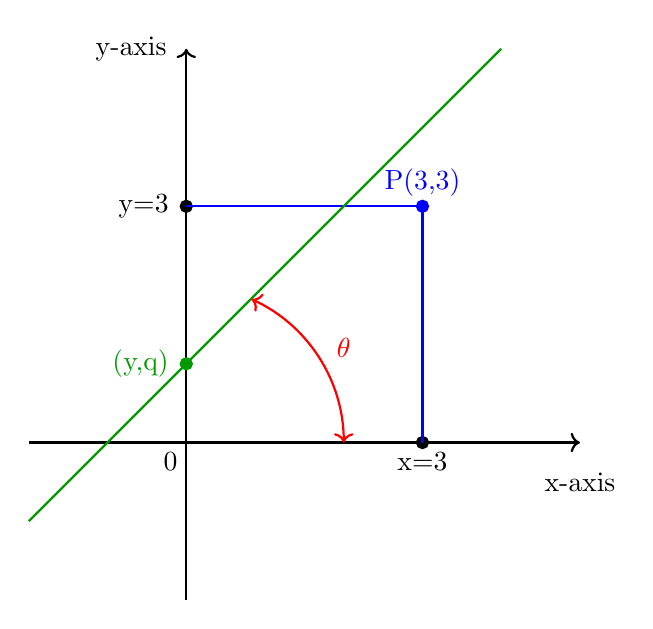
\begin{tikzpicture}
        \definecolor{darkgreen}{rgb}{0.0, 0.6, 0.0}

        \draw[thick][->] (-2,0) -- (5,0);
        \draw[thick][->] (0,-2) -- (0,5);
        \node at (5,-.5) {x-axis};
        \node at (-.7,5) {y-axis};
        \draw[fill, thick] (3,0) circle (2pt);
        \node[below] at (3,0) {x=3};
        \draw[fill, thick] (0,3) circle (2pt);
        \node[left] at (-.1,3) {y=3};
        \draw[blue, thick] (3,0) -- (3,3);
        \draw[blue,thick] (0,3) -- (3,3);
        \draw[fill, blue, thick] (3,3) circle (2pt);
        \node[blue, above] at (3,3) {P(3,3)};
        \node[below] at (-0.2,0) {0};
        
        \draw[darkgreen, thick] (-2,-1) -- (4,5);
        \draw[fill, darkgreen, thick] (0,1) circle (2pt);
        \node[darkgreen, left] at (-0.1,1) {(y,q)};

        \draw[red, thick, <->] (2,0) arc[start angle=0,end angle=65.5,radius=2];
        \node[red] at (2,1.2) {$\theta$};

    \end{tikzpicture}
\end{center}

\subsection{Straight line}
Let A and B be any two distinct points, then there is one and only one
line passing through A and B.

\subsection{Slope-intercept equation}
Let $m,q \in \mathbb{R}$, then
\figbox{$y=mx+q$}

\begin{itemize}
    \item $m$: slope;
    \item $q$: vertical intercept.
\end{itemize}

\subsubsection{Slope}
The slope of a line can be calculated with the equation
\figbox{$m=\dfrac{y_B-y_A}{x_B-x_A}=\dfrac{\Delta y}{\Delta x} = \tan{(\theta)}$}

We have three different slope outcomes:
\begin{itemize}
    \item $m>0$, the line is increasing;
    \item $m=0$, the line is stable;
    \item $m<0$, the line is decreasing. 
\end{itemize}

\wrn{This works only if $x_B \neq x_A$.}

\subsubsection{Drawing}
\begin{center}
    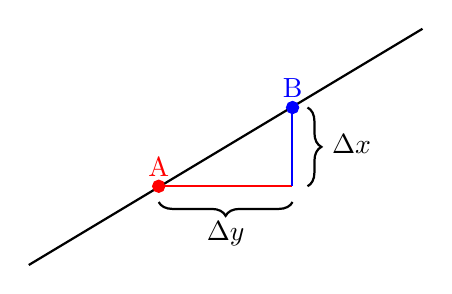
\begin{tikzpicture}
        \draw[thick] (0,0) -- (5,3);
        \draw[fill, thick, red] (1.65,1) circle (2pt);
        \node[above, red] at (1.65,1) {A};
        \draw[fill, thick, blue] (3.35,2) circle (2pt);
        \node [above, blue] at (3.35, 2) {B};

        %slope
        \draw[thick, red] (1.65,1) -- (3.34,1);
        \draw[thick, blue] (3.34,2) -- (3.34,1);

        %braces
        \draw[decorate,decoration={brace,amplitude=5pt},thick] (3.54,2) -- (3.54,1);
        \node at (4.1,1.53) {$\Delta x$};
        \draw[decorate,decoration={brace,amplitude=5pt},thick] (3.35,0.8) -- (1.65,0.8);
        \node at (2.5,0.4) {$\Delta y$};
    \end{tikzpicture}
\end{center}

\subsection{Vertical lines}
The more the value of m increases, the closer the line will get to the vertical,
without ever reaching it.

Let $c \in \mathbb{R}$, then $x=c$.

Vertical lines cannot be written as a function.

\section{Equation of a line}
Let $m,x_A,y_A \in \mathbb{R}$ and $A(x_A, y_A)$, then
\figbox{$y-y_A=m(x-x_A)$}

e.g.: Find the line with $m=-1$ and $A(2,-1)$.
\[
    y-1=-1(x+2) \Rightarrow y=-x+1
\]
\hspace{.75cm} Points: $A(2,-1);\ B(0,1)$


\begin{center}
    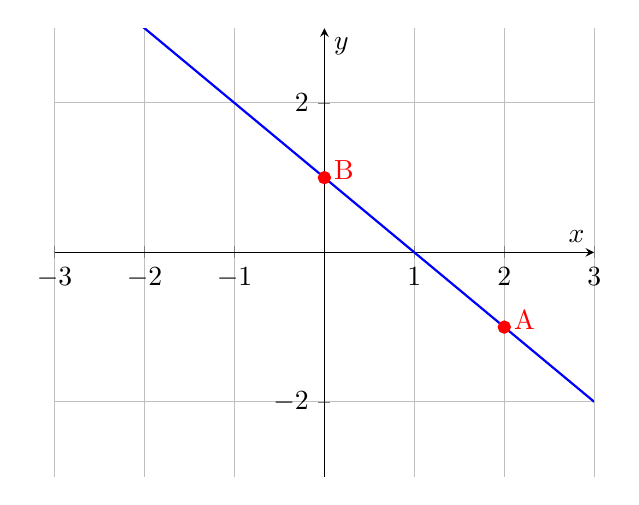
\begin{tikzpicture}
        \begin{axis}[
                axis lines = middle,
                xlabel = $x$,
                ylabel = $y$,
                grid = both,
                xmin=-3, xmax=3,
                ymin=-3, ymax=3,
                domain=-3:3
            ]
            \addplot[color=blue, thick] {-x + 1};
            \draw[fill, red, thick] (2,-1) circle (2pt);
            \node[right,red] at (2,-.9) {A};
            \draw[fill,red,thick] (0,1) circle (2pt);
            \node[right,red] at (0,1.1) {B};
        \end{axis}
    \end{tikzpicture}
\end{center}

\subsection{General equation in a cartesian diagram}
\figbox{$ax+by+c=0$}

\rem{\begin{itemize}
    \item All the lines can be described with this kind of equation;
    \item When $b=0$, $a \neq 0$, then $ax=-c \Rightarrow x=\dfrac{-c}{a} \in \mathbb{R}$;
    \item When $b \neq 0$, then $y=-\dfrac{a}{b}x -\dfrac{c}{b}$,
        where $m=-\dfrac{a}{b}$ and $q=-\dfrac{c}{b}$.
\end{itemize}}

\newpage
\section{Increasing and decreasing functions}
Let $f:[a,b] \longrightarrow \mathbb{R}$

\nots{if your replace $[a,b]$ with $\mathbb{R}$, you obtain the definition in the whote $\mathbb{R}$.}

\subsection{Increasing functions}
\begin{itemize}
    \item $f$ is increasing if $\forall x_1,x_2 \in [a,b] \sht x_2>x_1$, then $f(x_2)\geq f(x_1)$;
    \item $f$ is strictly increasing if $\forall x_1,x_2 \in [a,b] \sht x_2>x_1$, then $f(x_2)>f(x_1)$.
\end{itemize}

\subsection{Decreasing functions}
\begin{itemize}
    \item $f$ is decreasing if $\forall x_1,x_2 \in [a,b] \sht x_2>x_1$, then $f(x_2)\leq f(x_1)$;
    \item $f$ is strictly decreasing if $\forall x_1,x_2 \in [a,b] \sht x_2>x_1$, then $f(x_2)<f(x_1)$.
\end{itemize}

\section{Inverse function}
Let's take any two sets $A$ and $B$.

A function $f: A \rightarrow B$ is invertible if there exists another
function $f^{-1}: B \rightarrow A$, called the inverse function, such that:

\figbox{\begin{minipage}{3.6cm}
    $\forall x \in A,\ f^{-1}(f(x)) = x$ \vspace*{-.25cm}\\
    $\forall y \in B,\ f(f^{-1}(y)) = y$
\end{minipage}}

\wrn{A function is invertible if and only if it is bijective.}

\subsection{Facts about inverse functions}
\pph{1)}
Let $f:D\rightarrow \mathbb{R}$

$f$ is invertible in $D$ when:
\begin{itemize}
    \item $f$ is strictly increasing;
    \item $f$ is strictly decreasing.
\end{itemize}

\pph{2)}
Let $f:D \rightarrow \mathbb{R}$

$f$ is invertible when $f^{-1}:$ Im$(f) \rightarrow D$.

\newpage
\part{Week 3}
\section{Polynomial function}
\subsection{Expressions, terms and factors}
\subsubsection{Expressions}
An expression is any formula containing numbers, variables, operations, and
brackets.
\figbox{$y=ax^2+bx\cdot c$}

\subsubsection{Terms}
A term is any part of the expression separated by ``$+$'' or ``$-$''.
\figbox{$y = \underbrace{ax^2}_{term} + \underbrace{bx \cdot c}_{term}$}

\subsubsection{Factors}
Each term can be split into a product of factors.
\figbox{$x \cdot y \cdot (a-b) \cdot 24 = x \cdot y \cdot (a-b) \cdot 2 \cdot 2 \cdot 2 \cdot 3$}

\underline{Notice}: the process of splitting a term into several factors is called ``factorization''.\\
\phantom{} \hspace{1cm} The goal of a factorization is to factorize an expression as much as possible.

\section{Common factor}
Any expression made of terms is composed of several factors.
\figbox{$x^2+x^3+x= x(x+x^2+1),\ \forall x \in \mathbb{R}$}

\section{Notable products}
\begin{itemize}
    \item $(a+b)^2=a^2+2ab+b^2$ (square of a binomial);
    \item $(a-b)^2=a^2-2ab+b^2$ (square of a binomial);
    \item $(a-b)(a+b)=a^2-b^2$ (difference of squares);
    \item $(a+b)(a^2-ab+b^2)=a^3+b^3$ (sum of cubes);
    \item $(a-b)(a^2+ab+b^2)=a^3-b^3$ (difference of cubes).
\end{itemize}

\underline{Remark}: notable products are useful to factorize expressions when we don't know a common factor.

\section{Classification of polynomials}
Polynomials can be classified using two criteria: 
\begin{enumerate}
    \item the number of terms;
    \item the degree of the polynomial.
\end{enumerate}
\begin{equation*}
    \begin{aligned}
        &\begin{array}{|c|c|l|c|}
        \hline \text { Number of Terms } & \text { Name } & \text { Example } & \text { Comment } \\
        \hline \text { One } & \text { Monomial } & ax^2 & \text { Mono means ``one'' in Greek } \\
        \hline \text { Two } & \text { Binomial } & ax^2-b x & \text { Bi means ``two'' in Latin } \\
        \hline \text { Three } & \text { Trinomial } & ax^2-b x+c & \text { Tri means ``three'' in Greek } \\
        \hline \text { Four or more } & \text { Polynomial } & a x^3-b x^2+c x-d & \text { Poly means ``many'' in Greek } \\
        \hline
        \end{array}
    \end{aligned}
\end{equation*}

\subsection{Definition}
Let $n \in \mathbb{N^*}$, then a polynomial is the sum or difference of n-monomials. 

\subsection{Degree}
The degree of a polynomial is the largest exponent of its monomials.

\subsubsection{Monomials}
The degree of a monomial is the sum of all the exponents of all the variables.

$p(x)=x^2+1 \rightarrow$ the degree is 2.

$\forall x \in \mathbb{R},\ p(0)=0^2+1=1 \rightarrow$ A constant term, like 1, is a polynomial with degree 0.

\subsubsection{Polynomials}
The degree of a polynomial is the highest of all the degrees of all the
monomials which compose the polynomial.

$p(x)=x^3+1+x^5+x^21 \rightarrow \deg(p(x))=21$\\

Let $a,b,c,d,x,y$ be variables, then:

$q(a,b,c,d,x,y)=12 \underbrace{abcd}_{\deg=4} - 31x^3+2xy \rightarrow \deg(q(x))=4$ 

\underline{Notation}: Let $f(x)=ax^2+bx+c$,\ $a$, $b$ and $c$ are called coefficients.\\
The coefficient of the monomial with highest degree is called \textbf{leading coefficient}.

\section{Symmetrical functions}
Let $y = kx^n$, then we plot:
\subsection{$n$ odd}
\figbox{$f(-x)=-f(x), \quad \forall x \in \mathbb{R}$}

\subsubsection{Graph examples}
\begin{figure*}[htbp!]
    \centering
    \begin{subfigure}{0.45\textwidth}
        \centering
        \begin{tikzpicture}[scale=.95]
            \begin{axis}[
                domain=-2:2,
                samples=100,
                axis lines=middle,
                xlabel=$x$, ylabel={$y$},
            ]
            \addplot[color=blue, thick]{(x/2)^3};
            \end{axis}
        \end{tikzpicture}
        \caption*{$k > 0$}
    \end{subfigure}
    \hfill
    \begin{subfigure}{0.45\textwidth}
        \centering
        \begin{tikzpicture}[scale=.95]
            \begin{axis}[
                domain=-2:2,
                samples=100,
                axis lines=middle,
                xlabel=$x$, ylabel={$y$},
            ]
            \addplot[color=red, thick]{-(x/2)^3};
            \end{axis}
        \end{tikzpicture}
        \caption*{$k < 0$}
    \end{subfigure}
\end{figure*}

\newpage
\subsection{$n$ even}
\figbox{$f(-x)=f(x), \quad \forall x \in \mathbb{R}$}

\subsubsection{Graph examples}
\begin{figure}[htbp]
    \centering
    \begin{subfigure}{0.45\textwidth}
        \centering
        \begin{tikzpicture}[scale=.95]
            \begin{axis}[
                domain=-2:2,
                samples=100,
                axis lines=middle,
                xlabel=$x$, ylabel={$y$},
            ]
            \addplot[color=blue, thick]{(x/2)^2};
            \end{axis}
        \end{tikzpicture}
        \caption*{$k > 0$ \\ Concave up}
    \end{subfigure}
    \hfill
    \begin{subfigure}{0.45\textwidth}
        \centering
        \begin{tikzpicture}[scale=.95]
            \begin{axis}[
                domain=-2:2,
                samples=100,
                axis lines=middle,
                xlabel=$x$, ylabel={$y$},
            ]
            \addplot[color=red, thick]{-(x/2)^2};
            \end{axis}
        \end{tikzpicture}
        \caption*{$k < 0$\\Concave down}
    \end{subfigure}
\end{figure}

\defs{\begin{itemize}
    \item a function $y=f(x)$ is called \textbf{odd} if it is symmetric with
    respect to the origin;
    \item a function $y=f(x)$ is called \textbf{even} if it is symmetric
    with respect to the y-axis.
\end{itemize}}

\subsection{General case}
Let $y=p(x)$, where $p(x)$ is any polynomial with real coefficients:
\figbox{$p(x)=a_n \cdot x^n + a_{n-1} \cdot x^{n-1} + a_{n-2} \cdot x^{n-2} + ... + a_{2} \cdot x^{2} + a_{1} \cdot x^{1} + a_{0}$}

where:
\begin{itemize}
    \item $n \in \mathbb{N}$;
    \item $n=\deg(p(x))$;
    \item $a_n=$ leading coefficient.
\end{itemize}

\figbox{\large $\displaystyle p(x)=\sum^{n}_{i=0} a_i \cdot x^i$}

\subsection{Symmetry of a polynomial}
Let $y=p(x)$ be a polynomial function, then:
\pph{1)}
$y=p(x)$ is odd iff all the degrees of all the terms of
$p(x)$ are odd;

\pph{2)}
$y=p(x)$ is even iff all the degrees of all the terms of
$p(x)$ are even;

\pph{3)}
$y=p(x)$ has mixed degrees, $p(x)$ is neither odd nor even.

\newpage
\section{Intersection with axis}
\subsection{Vertical intersection}
Let $y=f(x)$ be any function, then we solve for $y$:
\figbox{$\begin{cases}
    x = 0 \\
    y=f(0)
\end{cases}$}

\subsection{Zeros of a function}
Let $y=f(x)$ be any function, then we solve for $x$:
\figbox{$\begin{cases}
    y = 0 \\
    0 = f(x)
\end{cases}$}

\subsection{Graph example}
\begin{center}
    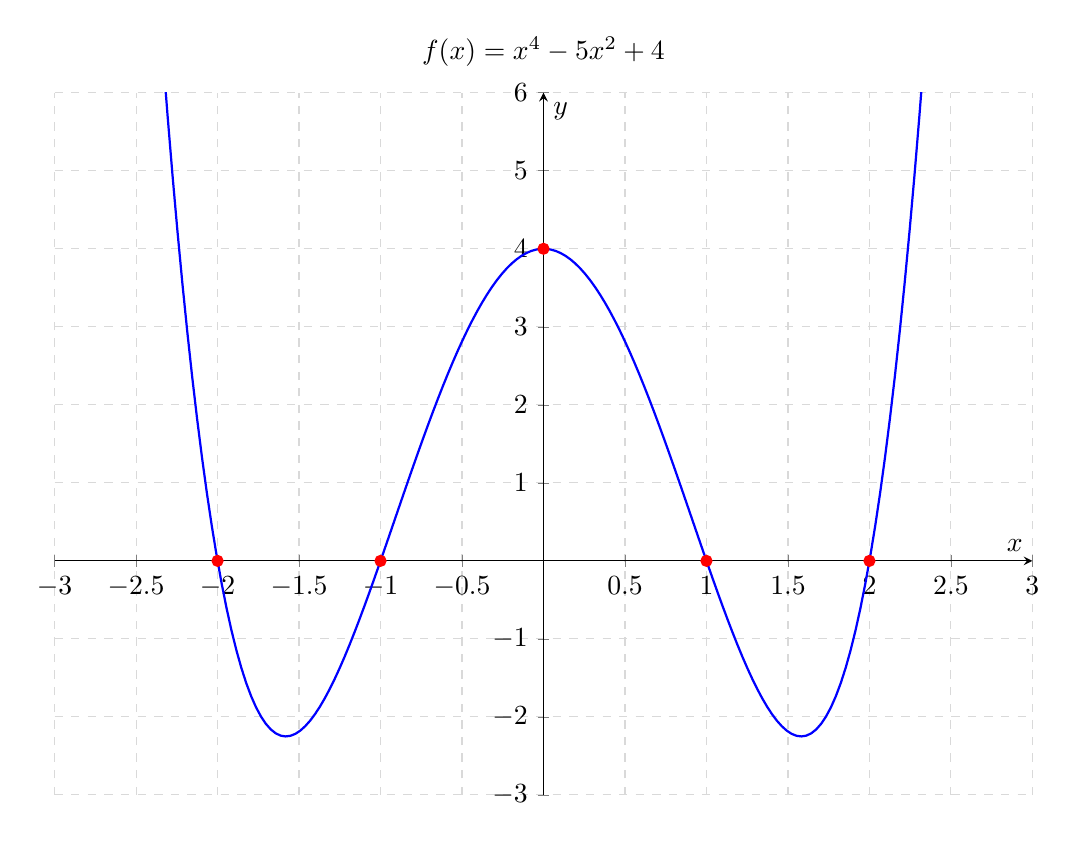
\begin{tikzpicture}
        \begin{axis}[
          title = {$f(x)=x^4-5x^2+4$},
          axis lines = middle,
          xlabel = $x$,
          ylabel = $y$,
          xmin = -3, xmax = 3,
          ymin = -3, ymax = 6,
          samples = 200,
          domain = -3:3,
          clip = true,
          grid = both,
          grid style = {dashed, gray!30},
          width = 14cm,
          height = 10.5cm,
        ]
        \addplot [blue, thick] {x^4 - 5*x^2 + 4};
        
        \addplot [
          only marks,
          mark=*,
          mark options={color=red},
        ] coordinates {
          (-2, 0) (-1, 0) (1, 0) (2, 0)
        };
        
        \addplot [
          only marks,
          mark=*,
          mark options={color=red},
        ] coordinates {
          (0, 4)
        };
        \end{axis}
    \end{tikzpicture}      
\end{center} 

\newpage
\section{Dominant elements in a function approaching $\pm \infty$}
As $x$ approaches $\pm \infty$, the term with the highest degree in a
polynomial function dominates the behavior of the function.
\figbox{$p(x)$ has, as a dominant, the element $a_n$ with the highest degree $x^n$}

\subsection{Order of dominance}
\subsubsection{Approaching to +$\infty$}
Let $n \in \mathbb{N},\ m \in \mathbb{N},\ 2<n<m$, then:

\figbox{$\ln(x) < x < x^n < x^m < n^x < m^x < x^x$}

In these cases, we always have $x \rightarrow +\infty \Rightarrow p(x)\rightarrow +\infty$

\subsubsection{Approaching to -$\infty$}
Let $\lambda > 2$ and odd,\ $k > 2$ and even.

\figbox{
  \begin{minipage}{3.25cm}
    $x^\lambda < -x^2 < x^1 < 0$ \\
    $-x^k < -x^2 < x^1 < 0$
  \end{minipage}
}

Functions like $x^\lambda$ (with $\lambda$ odd) and $-x^k$ (with $k$ even)
both approach $-\infty$, but at different rates.

\subsubsection{Dominance in rational functions}
When the dominant element is at the numerator:
\figbox{$\dm \lim_{x \to \infty} \dfrac{x^n}{x^{n-1}} = \infty$}

When the dominant element is at the denominator:
\figbox{$\dm \lim_{x \to \infty} \dfrac{x^{n-1}}{x^n} = 0$}

When we have the same degree either in the numerator and in the denominator:
\figbox{$\dm \lim_{x \to \infty} \dfrac{ax^n}{bx^n} = \dfrac{a}{b}$}

\defs{\textbf{horizontal asymptote} appears when $x$ approaches to $\infty$,
which implies that $y$ approaches to a number $A$ different from $\pm \infty$}










\end{document}
